\documentclass[a4paper,11pt]{article}
\input{/home/tof/Documents/Cozy/latex-include/preambule_doc.tex}
\input{/home/tof/Documents/Cozy/latex-include/preambule_commun.tex}
\newcommand{\showprof}{show them}  % comment this line if you don't want to see todo environment
\setlength{\fboxrule}{0.8pt}
\fancyhead[L]{\fbox{\Large{\textbf{Routage 01}}}}
\fancyhead[C]{\textbf{Principe du routage}}
\newdate{madate}{10}{09}{2020}
%\fancyhead[R]{\displaydate{madate}} %\today
%\fancyhead[R]{Seconde - SNT}
%\fancyhead[R]{Première - NSI}
\fancyhead[R]{Terminale - NSI}
\fancyfoot[L]{\vspace{1mm}Christophe Viroulaud}
\AtEndDocument{\label{lastpage}}
\fancyfoot[C]{\textbf{Page \thepage/\pageref{lastpage}}}
\fancyfoot[R]{\includegraphics[width=2cm,align=t]{/home/tof/Documents/Cozy/latex-include/cc.png}}

\begin{document}
\section{Problématique}
Le réseau internet permet de communiquer avec n'importe quelle machine connectée. En juin 2020 on dénombrait 1,78 milliards de sites web dans le monde.
\begin{center}
    \framebox{Comment retrouver une machine précise dans le réseau?}
\end{center}
\section{Adresse IP}
Sur un réseau chaque machine est repérée par son \emph{adresse IP}. L'\textbf{Internet Protocol} version 4 (IPv4) est peu à peu remplacée par la version 6 pour pallier la pénurie d'adresses. Une adresse IPv4 est composée de 4 octets.
\begin{center}
    Un exemple: \large{192.168.10.3}
\end{center}
Une adresse IP est accompagnée de son masque de sous-réseau. Il permet de déterminer le réseau auquel appartient la machine.
\begin{center}
    \begin{tabular}{ccccc}
        adresse IP & 192 & 168 & 10  & 3 \\
        masque     & 255 & 255 & 255 & 0 \\
    \end{tabular}
\end{center}
Pour connaître le réseau on convertit les adresses en binaire et on applique une porte logique \emph{AND}.
\begin{center}
    \begin{tabular}{ccccc}
        adresse IP & 11000000 & 10101000 & 00001010 & 00000011 \\
        masque     & 11111111 & 11111111 & 11111111 & 00000000 \\
        réseau     & 11000000 & 10101000 & 00001010 & 00000000 \\
    \end{tabular}
\end{center}

\begin{aretenir}[]
    On note une adresse IP avec son masque de sous-réseau. Le nombre après / correspond au nombre de 1 du masque (notation \emph{CIDR} - (Classless Inter-Domain Routing)).
    \begin{center}
        192.168.10.3/24
    \end{center}
    Les 24 premiers bits correspondent au réseau.
    \begin{commentprof}
        Il y a donc $2^{32-24}$ adresses disponibles dans le réseau (- adresse de réseau et adresse de broadcast). adresse du réseau: 192.168.10.0; possibilité de créer des sous-réseaux en "augmentant" le masque
    \end{commentprof}
\end{aretenir}

\begin{activite}
    \begin{enumerate}
        \item Donner le réseau auquel appartient l'adresse 10.103.10.2/12
        \item Combien d'adresses peut-on créer dans ce réseau?
        \item Ouvrir un terminal et taper la commande (code \ref{ip}).
        \begin{center}
            \begin{lstlisting}[language=bash]
# a pour adresse, 4 pour n'avoir que les IPv4
ip -4 a
            \end{lstlisting}
            \captionof{code}{Adresse IPv4}
            \label{ip}
        \end{center}

        \item Quelle est l'adresse de la machine?
        \item Quelle est l'adresse du réseau?
    \end{enumerate}
\end{activite}
\begin{commentprof}
adresse de broadcast; adresse 169.254... = quand machine n'obtient pas adresse via DHCP, elle s'en crée une
\end{commentprof}
\section{Structure maillée}
Connaître l'adresse IP du destinataire est une première étape, mais il faut maintenant pouvoir le repérer dans le réseau. Il est illusoire de penser que chaque machine connaisse la totalité de la structure du réseau.

Un réseau est structuré autour des \textbf{routeurs}. Ces machines relaient les paquets de données jusqu'au destinataire. On distingue deux catégories:
\begin{itemize}
    \item Les routeurs d'accès permettent d'accéder à un réseau ou assure la connexion entre deux réseaux. La box d'une maison est un routeur d'accès.
    \item Les routeurs internes forment la topologie du réseau. Les prestataires (Orange, Free \dots) créent un réseau accessible via la box. 
\end{itemize}
\begin{center}
    \centering
    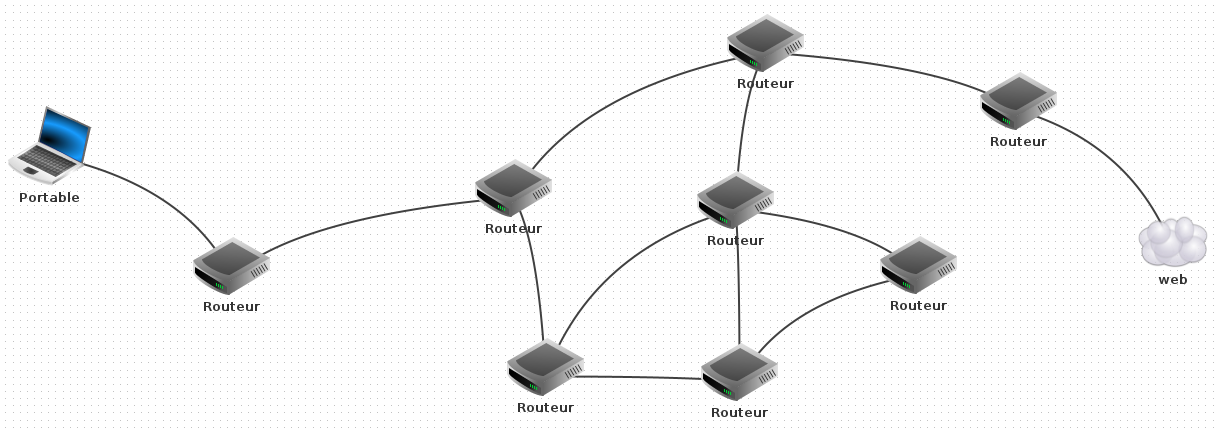
\includegraphics[width=15cm]{ressources/reseau.png}
    \captionof{figure}{Topologie d'un réseau}
    \label{reseau}
\end{center}
\begin{activite}
\begin{enumerate}
    \item Sur la figure \ref{reseau}, repérer les routeurs d'accès, les routeurs internes.
    \item Installer le paquet \emph{traceroute}
    \begin{center}
        \begin{lstlisting}[language=bash]
sudo apt install traceroute
        \end{lstlisting}
        \captionof{code}{Installation d'un paquet}
        \label{ip}
    \end{center}
    \item Taper la commande (code \ref{trace}).
    \begin{center}
        \begin{lstlisting}[language=bash]
traceroute fr.wikipedia.org
        \end{lstlisting}
        \captionof{code}{Tracer le chemin suivi vers une destination}
        \label{trace}
    \end{center}
\end{enumerate}
\end{activite}
\begin{commentprof}
Le serveur destinataire rejette les paquets UDP (User Datagram Protocol) (n'accepte que les TCP - Transmission Control Protocol).

L'option -I de traceroute permet d'envoyer des paquets avec le protcole ICMP (Internet Control Message Protocol) = ping
\end{commentprof}
\end{document}